% ==============================================================================
% ฝาปกหน้า Smartphone UI เสมือนจริง (Virtual Mobile Viewfinder Cover Architecture)
% ตำราวิชาการ: การออกแบบและพัฒนาแอปพลิเคชัน วิเคราะห์โรคและความสมบูรณ์ของไม้ผลด้วย AI +Deep Learning
% มาตรฐานมหาวิทยาลัยราชภัฏรำไพพรรณี (Zero-Colon Rule ปราศจากเครื่องหมายทวิภาค 100%)
% ==============================================================================
\begin{titlepage}
\newgeometry{left=0mm, right=0mm, top=0mm, bottom=0mm}

\begin{tikzpicture}[remember picture, overlay]
  % 1. พื้นหลังไล่ระดับสีหรูหราทันสมัย (Dark Forest Green to Deep Emerald Tech)
  \fill[top color=rbruDeepForest, bottom color=black]
    (current page.south west) rectangle (current page.north east);

  % แถบขอบเย็บเล่ม 1.5 นิ้ว ด้านซ้าย
  \fill[black, opacity=0.35]
    (current page.north west) rectangle ++(38.1mm, -\paperheight);

  % 2. แถบหัวกระดาษสถาบันวิชาการ
  \node[anchor=north west] at ([xshift=44mm, yshift=-16mm]current page.north west) {
    \begin{minipage}{150mm}
      \begin{flushleft}
        {\fontsize{10pt}{14pt}\selectfont\bfseries\color{rbruGold} หน่วยวิเคราะห์-ติดตามคุณภาพดินและสภาพอากาศเชิงพื้นที่}\\[1mm]
        {\fontsize{8.5pt}{12pt}\selectfont\color{white!75} คณะวิทยาศาสตร์และเทคโนโลยี มหาวิทยาลัยราชภัฏรำไพพรรณี}
      \end{flushleft}
    \end{minipage}
  };

  % 3. ชื่อเอกสารวิชาการขนาดใหญ่พิเศษ (Hero Title)
  \node[anchor=north west] at ([xshift=44mm, yshift=-33mm]current page.north west) {
    \begin{minipage}{152mm}
      \begin{flushleft}
        \color{white}
        {\fontsize{26pt}{33pt}\selectfont\bfseries การออกแบบและพัฒนาแอปพลิเคชัน}\\[2mm]
        {\fontsize{23pt}{30pt}\selectfont\bfseries วิเคราะห์โรคและความสมบูรณ์ของไม้ผล}\\[2mm]
        {\fontsize{24pt}{31pt}\selectfont\bfseries\color{rbruGold} ด้วย AI +Deep Learning}\\[4mm]
        {\fontsize{10.5pt}{14pt}\selectfont\bfseries\color{white!90}
        DESIGN AND DEVELOPMENT OF AN APPLICATION FOR FRUIT TREE PATHOLOGY}\\[1mm]
        {\fontsize{9.5pt}{13pt}\selectfont\bfseries\color{white!75}
        AND HEALTH ASSESSMENT USING AI + DEEP LEARNING}
      \end{flushleft}
    \end{minipage}
  };

  % 4. หน้าจอสมาร์ทโฟนเสมือนจริง (Smartphone Screen Frame with PR Image)
  \node[anchor=center] at ([xshift=20mm, yshift=-26mm]current page.center) {
    \begin{tikzpicture}
      % ตัวเครื่องสมาร์ทโฟนขอบมนสีไทเทเนียมเข้ม
      \draw[draw=white!40, fill=black!85, rounded corners=22pt, line width=2.4pt]
        (-5.2, -4.6) rectangle (5.2, 4.6);

      % แถบ Notch และกล้องหน้าสมาร์ทโฟน
      \fill[fill=black, rounded corners=6pt] (-1.6, 4.25) rectangle (1.6, 4.55);
      \fill[fill=white!30] (1.0, 4.40) circle (1.8pt);

      % ภาพใบไม้ดิจิทัลวงจรอิเล็กทรอนิกส์และโครงข่ายประสาทเทียม (Digital Leaf AI Art)
      \node at (0, 0.1) {
        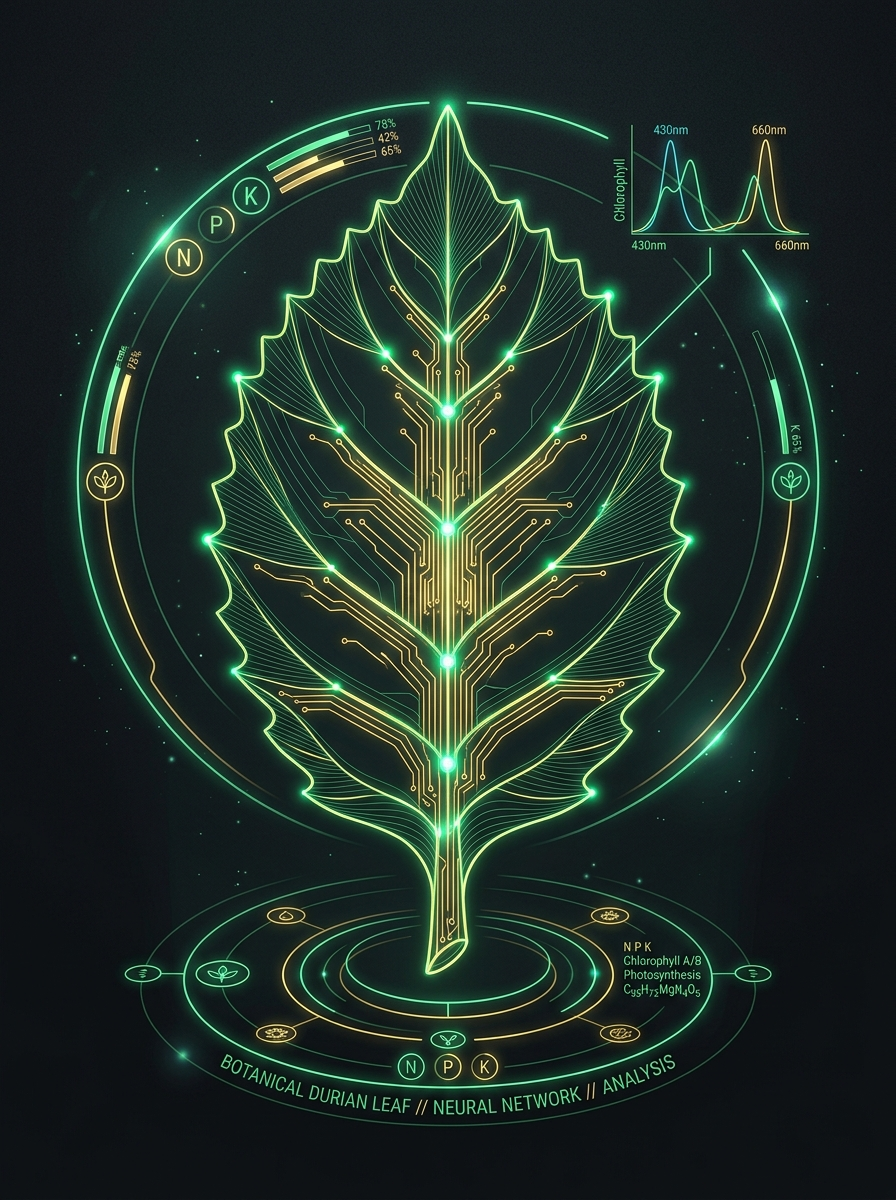
\includegraphics[width=9.8cm, height=8.2cm, keepaspectratio]{figures/durian_digital_leaf_art.jpg}
      };

      % กรอบการตรวจจับเล็งรอยโรคและใบไม้ (Targeting Reticle)
      \draw[draw=rbruGreen, line width=1.5pt, dashed] (-3.8, -2.4) rectangle (3.8, 2.6);
      \fill[fill=rbruGreen] (-3.8, 2.6) circle (3pt);
      \fill[fill=rbruGreen] (3.8, 2.6) circle (3pt);
      \fill[fill=rbruGreen] (-3.8, -2.4) circle (3pt);
      \fill[fill=rbruGreen] (3.8, -2.4) circle (3pt);

      % ป้ายสถิติ AI สดบนจอสมาร์ทโฟน (Zero-Colon Rule ปราศจากเครื่องหมายทวิภาค)
      \node[anchor=north west, fill=black!85, text=white, rounded corners=4pt, inner sep=4pt]
        at (-3.6, 2.4) {
          \fontsize{7.5pt}{10pt}\selectfont\bfseries\color{rbruGreen} LIVE AI 30 FPS \color{white} \textbar\ DEEP LEARNING DUAL-HEAD TFLITE
        };

      \node[anchor=south west, fill=black!85, text=white, rounded corners=4pt, inner sep=5pt]
        at (-3.6, -2.2) {
          \fontsize{8.5pt}{11pt}\selectfont
          \textbf{ผลวินิจฉัย} ใบปกติสมบูรณ์ (98.5\%)\\[1mm]
          \textbf{โภชนาการ} SPAD 48.5 \textbar\ N 2.50\% \textbar\ K 1.85\% \textbar\ Mg 0.42\%
        };

      % ปุ่มชัตเตอร์สมาร์ทโฟน
      \draw[draw=white!70, line width=1.8pt] (0, -3.8) circle (8pt);
      \fill[fill=white] (0, -3.8) circle (6pt);
    \end{tikzpicture}
  };

  % 5. ข้อมูลผู้จัดทำและปีพิมพ์ท้ายปก (Zero-Colon Rule)
  \node[anchor=south west] at ([xshift=44mm, yshift=16mm]current page.south west) {
    \begin{minipage}{152mm}
      \begin{flushleft}
        \color{white!80}
        {\fontsize{10.5pt}{15pt}\selectfont\bfseries ผู้ช่วยศาสตราจารย์ ดร.ชีวะ ทัศนา และคณะนักวิจัย}\\[1mm]
        {\fontsize{9pt}{13pt}\selectfont\color{white!75} หน่วยวิเคราะห์-ติดตามคุณภาพดินและสภาพอากาศเชิงพื้นที่}\\[1mm]
        {\fontsize{9pt}{13pt}\selectfont\color{white!65} คณะวิทยาศาสตร์และเทคโนโลยี มหาวิทยาลัยราชภัฏรำไพพรรณี}\\[1mm]
        {\fontsize{9pt}{13pt}\selectfont\color{rbruGold} เอกสารคู่มือวิชาการและวิจัยฉบับสมบูรณ์ พุทธศักราช 2569}
      \end{flushleft}
    \end{minipage}
  };
\end{tikzpicture}

\restoregeometry
\end{titlepage}
